% Created by tikzDevice version 0.12.3.1 on 2022-04-17 13:34:10
% !TEX encoding = UTF-8 Unicode
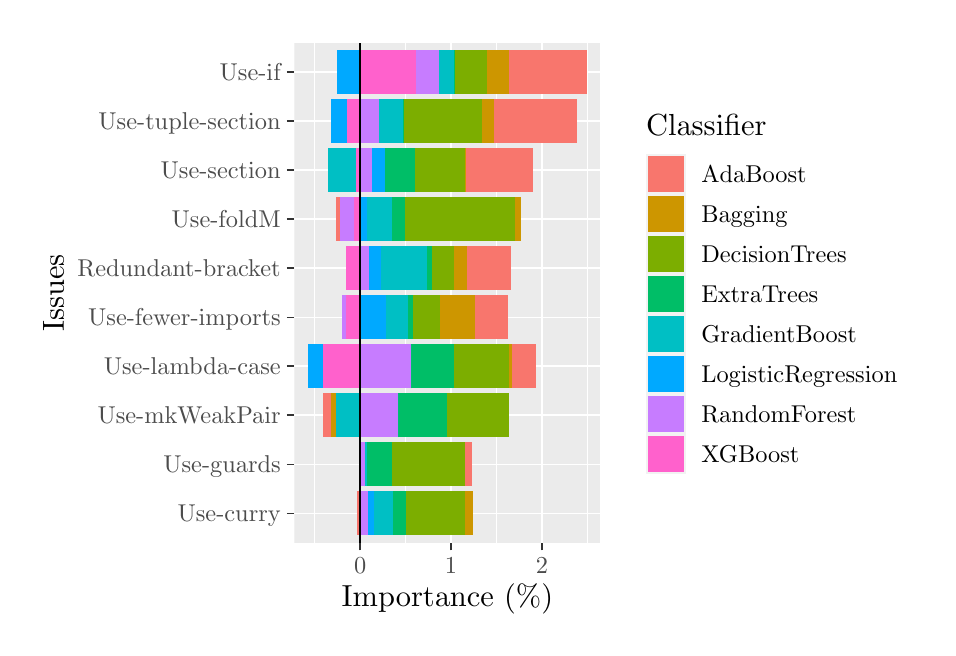
\begin{tikzpicture}[x=1pt,y=1pt]
\definecolor{fillColor}{RGB}{255,255,255}
\path[use as bounding box,fill=fillColor,fill opacity=0.00] (0,0) rectangle (325.21,216.81);
\begin{scope}
\path[clip] (  0.00,  0.00) rectangle (325.21,216.81);
\definecolor{drawColor}{RGB}{255,255,255}
\definecolor{fillColor}{RGB}{255,255,255}

\path[draw=drawColor,line width= 0.6pt,line join=round,line cap=round,fill=fillColor] (  0.00,  0.00) rectangle (325.21,216.81);
\end{scope}
\begin{scope}
\path[clip] ( 96.38, 30.69) rectangle (206.96,211.31);
\definecolor{fillColor}{gray}{0.92}

\path[fill=fillColor] ( 96.38, 30.69) rectangle (206.96,211.31);
\definecolor{drawColor}{RGB}{255,255,255}

\path[draw=drawColor,line width= 0.3pt,line join=round] (103.70, 30.69) --
	(103.70,211.31);

\path[draw=drawColor,line width= 0.3pt,line join=round] (136.56, 30.69) --
	(136.56,211.31);

\path[draw=drawColor,line width= 0.3pt,line join=round] (169.41, 30.69) --
	(169.41,211.31);

\path[draw=drawColor,line width= 0.3pt,line join=round] (202.26, 30.69) --
	(202.26,211.31);

\path[draw=drawColor,line width= 0.6pt,line join=round] ( 96.38, 41.31) --
	(206.96, 41.31);

\path[draw=drawColor,line width= 0.6pt,line join=round] ( 96.38, 59.02) --
	(206.96, 59.02);

\path[draw=drawColor,line width= 0.6pt,line join=round] ( 96.38, 76.73) --
	(206.96, 76.73);

\path[draw=drawColor,line width= 0.6pt,line join=round] ( 96.38, 94.44) --
	(206.96, 94.44);

\path[draw=drawColor,line width= 0.6pt,line join=round] ( 96.38,112.14) --
	(206.96,112.14);

\path[draw=drawColor,line width= 0.6pt,line join=round] ( 96.38,129.85) --
	(206.96,129.85);

\path[draw=drawColor,line width= 0.6pt,line join=round] ( 96.38,147.56) --
	(206.96,147.56);

\path[draw=drawColor,line width= 0.6pt,line join=round] ( 96.38,165.27) --
	(206.96,165.27);

\path[draw=drawColor,line width= 0.6pt,line join=round] ( 96.38,182.98) --
	(206.96,182.98);

\path[draw=drawColor,line width= 0.6pt,line join=round] ( 96.38,200.69) --
	(206.96,200.69);

\path[draw=drawColor,line width= 0.6pt,line join=round] (120.13, 30.69) --
	(120.13,211.31);

\path[draw=drawColor,line width= 0.6pt,line join=round] (152.98, 30.69) --
	(152.98,211.31);

\path[draw=drawColor,line width= 0.6pt,line join=round] (185.84, 30.69) --
	(185.84,211.31);
\definecolor{fillColor}{RGB}{248,118,109}

\path[fill=fillColor] (174.01,192.72) rectangle (201.94,208.65);

\path[fill=fillColor] (168.42,175.01) rectangle (198.32,190.95);

\path[fill=fillColor] (158.24,157.30) rectangle (182.55,173.24);

\path[fill=fillColor] (111.59,139.59) rectangle (112.90,155.53);

\path[fill=fillColor] (158.90,121.88) rectangle (174.67,137.82);

\path[fill=fillColor] (161.53,104.18) rectangle (173.68,120.11);

\path[fill=fillColor] (175.00, 86.47) rectangle (183.54,102.40);

\path[fill=fillColor] (106.66, 68.76) rectangle (109.62, 84.70);

\path[fill=fillColor] (157.91, 51.05) rectangle (160.54, 66.99);

\path[fill=fillColor] (119.14, 33.34) rectangle (120.13, 49.28);
\definecolor{fillColor}{RGB}{205,150,0}

\path[fill=fillColor] (166.13,192.72) rectangle (174.01,208.65);

\path[fill=fillColor] (164.15,175.01) rectangle (168.42,190.95);

\path[fill=fillColor] (157.91,157.30) rectangle (158.24,173.24);

\path[fill=fillColor] (175.98,139.59) rectangle (178.28,155.53);

\path[fill=fillColor] (153.97,121.88) rectangle (158.90,137.82);

\path[fill=fillColor] (149.04,104.18) rectangle (161.53,120.11);

\path[fill=fillColor] (174.01, 86.47) rectangle (175.00,102.40);

\path[fill=fillColor] (109.62, 68.76) rectangle (111.59, 84.70);

\path[fill=fillColor] (119.80, 51.05) rectangle (120.13, 66.99);

\path[fill=fillColor] (157.91, 33.34) rectangle (160.87, 49.28);
\definecolor{fillColor}{RGB}{124,174,0}

\path[fill=fillColor] (154.30,192.72) rectangle (166.13,208.65);

\path[fill=fillColor] (135.90,175.01) rectangle (164.15,190.95);

\path[fill=fillColor] (139.84,157.30) rectangle (157.91,173.24);

\path[fill=fillColor] (136.23,139.59) rectangle (175.98,155.53);

\path[fill=fillColor] (146.08,121.88) rectangle (153.97,137.82);

\path[fill=fillColor] (139.19,104.18) rectangle (149.04,120.11);

\path[fill=fillColor] (153.97, 86.47) rectangle (174.01,102.40);

\path[fill=fillColor] (151.67, 68.76) rectangle (174.01, 84.70);

\path[fill=fillColor] (131.63, 51.05) rectangle (157.91, 66.99);

\path[fill=fillColor] (136.56, 33.34) rectangle (157.91, 49.28);
\definecolor{fillColor}{RGB}{0,190,103}

\path[fill=fillColor] (153.97,192.72) rectangle (154.30,208.65);

\path[fill=fillColor] (135.57,175.01) rectangle (135.90,190.95);

\path[fill=fillColor] (129.00,157.30) rectangle (139.84,173.24);

\path[fill=fillColor] (131.63,139.59) rectangle (136.23,155.53);

\path[fill=fillColor] (144.44,121.88) rectangle (146.08,137.82);

\path[fill=fillColor] (137.54,104.18) rectangle (139.19,120.11);

\path[fill=fillColor] (138.53, 86.47) rectangle (153.97,102.40);

\path[fill=fillColor] (133.93, 68.76) rectangle (151.67, 84.70);

\path[fill=fillColor] (122.76, 51.05) rectangle (131.63, 66.99);

\path[fill=fillColor] (131.96, 33.34) rectangle (136.56, 49.28);
\definecolor{fillColor}{RGB}{0,191,196}

\path[fill=fillColor] (148.71,192.72) rectangle (153.97,208.65);

\path[fill=fillColor] (127.03,175.01) rectangle (135.57,190.95);

\path[fill=fillColor] (108.63,157.30) rectangle (118.49,173.24);

\path[fill=fillColor] (122.76,139.59) rectangle (131.63,155.53);

\path[fill=fillColor] (127.69,121.88) rectangle (144.44,137.82);

\path[fill=fillColor] (129.33,104.18) rectangle (137.54,120.11);

\path[fill=fillColor] (138.53, 86.47) rectangle (138.53,102.40);

\path[fill=fillColor] (111.59, 68.76) rectangle (120.13, 84.70);

\path[fill=fillColor] (121.77, 51.05) rectangle (122.76, 66.99);

\path[fill=fillColor] (125.06, 33.34) rectangle (131.96, 49.28);
\definecolor{fillColor}{RGB}{0,169,255}

\path[fill=fillColor] (111.92,192.72) rectangle (120.13,208.65);

\path[fill=fillColor] (109.62,175.01) rectangle (115.53,190.95);

\path[fill=fillColor] (124.40,157.30) rectangle (129.00,173.24);

\path[fill=fillColor] (120.13,139.59) rectangle (122.76,155.53);

\path[fill=fillColor] (123.42,121.88) rectangle (127.69,137.82);

\path[fill=fillColor] (120.13,104.18) rectangle (129.33,120.11);

\path[fill=fillColor] (101.40, 86.47) rectangle (106.66,102.40);

\path[fill=fillColor] (133.93, 68.76) rectangle (133.93, 84.70);

\path[fill=fillColor] (121.77, 51.05) rectangle (121.77, 66.99);

\path[fill=fillColor] (123.09, 33.34) rectangle (125.06, 49.28);
\definecolor{fillColor}{RGB}{199,124,255}

\path[fill=fillColor] (140.17,192.72) rectangle (148.71,208.65);

\path[fill=fillColor] (120.13,175.01) rectangle (127.03,190.95);

\path[fill=fillColor] (120.13,157.30) rectangle (124.40,173.24);

\path[fill=fillColor] (112.90,139.59) rectangle (117.83,155.53);

\path[fill=fillColor] (120.13,121.88) rectangle (123.42,137.82);

\path[fill=fillColor] (113.56,104.18) rectangle (114.87,120.11);

\path[fill=fillColor] (120.13, 86.47) rectangle (138.53,102.40);

\path[fill=fillColor] (120.13, 68.76) rectangle (133.93, 84.70);

\path[fill=fillColor] (120.13, 51.05) rectangle (121.77, 66.99);

\path[fill=fillColor] (120.13, 33.34) rectangle (123.09, 49.28);
\definecolor{fillColor}{RGB}{255,97,204}

\path[fill=fillColor] (120.13,192.72) rectangle (140.17,208.65);

\path[fill=fillColor] (115.53,175.01) rectangle (120.13,190.95);

\path[fill=fillColor] (118.49,157.30) rectangle (120.13,173.24);

\path[fill=fillColor] (117.83,139.59) rectangle (120.13,155.53);

\path[fill=fillColor] (115.20,121.88) rectangle (120.13,137.82);

\path[fill=fillColor] (114.87,104.18) rectangle (120.13,120.11);

\path[fill=fillColor] (106.66, 86.47) rectangle (120.13,102.40);

\path[fill=fillColor] (120.13, 68.76) rectangle (120.13, 84.70);

\path[fill=fillColor] (120.13, 51.05) rectangle (120.13, 66.99);

\path[fill=fillColor] (120.13, 33.34) rectangle (120.13, 49.28);
\definecolor{drawColor}{RGB}{0,0,0}

\path[draw=drawColor,line width= 0.6pt,line join=round] (120.13, 30.69) -- (120.13,211.31);
\end{scope}
\begin{scope}
\path[clip] (  0.00,  0.00) rectangle (325.21,216.81);
\definecolor{drawColor}{gray}{0.30}

\node[text=drawColor,anchor=base east,inner sep=0pt, outer sep=0pt, scale=  0.88] at ( 91.43, 38.28) {Use-curry};

\node[text=drawColor,anchor=base east,inner sep=0pt, outer sep=0pt, scale=  0.88] at ( 91.43, 55.99) {Use-guards};

\node[text=drawColor,anchor=base east,inner sep=0pt, outer sep=0pt, scale=  0.88] at ( 91.43, 73.70) {Use-mkWeakPair};

\node[text=drawColor,anchor=base east,inner sep=0pt, outer sep=0pt, scale=  0.88] at ( 91.43, 91.41) {Use-lambda-case};

\node[text=drawColor,anchor=base east,inner sep=0pt, outer sep=0pt, scale=  0.88] at ( 91.43,109.11) {Use-fewer-imports};

\node[text=drawColor,anchor=base east,inner sep=0pt, outer sep=0pt, scale=  0.88] at ( 91.43,126.82) {Redundant-bracket};

\node[text=drawColor,anchor=base east,inner sep=0pt, outer sep=0pt, scale=  0.88] at ( 91.43,144.53) {Use-foldM};

\node[text=drawColor,anchor=base east,inner sep=0pt, outer sep=0pt, scale=  0.88] at ( 91.43,162.24) {Use-section};

\node[text=drawColor,anchor=base east,inner sep=0pt, outer sep=0pt, scale=  0.88] at ( 91.43,179.95) {Use-tuple-section};

\node[text=drawColor,anchor=base east,inner sep=0pt, outer sep=0pt, scale=  0.88] at ( 91.43,197.65) {Use-if};
\end{scope}
\begin{scope}
\path[clip] (  0.00,  0.00) rectangle (325.21,216.81);
\definecolor{drawColor}{gray}{0.20}

\path[draw=drawColor,line width= 0.6pt,line join=round] ( 93.63, 41.31) --
	( 96.38, 41.31);

\path[draw=drawColor,line width= 0.6pt,line join=round] ( 93.63, 59.02) --
	( 96.38, 59.02);

\path[draw=drawColor,line width= 0.6pt,line join=round] ( 93.63, 76.73) --
	( 96.38, 76.73);

\path[draw=drawColor,line width= 0.6pt,line join=round] ( 93.63, 94.44) --
	( 96.38, 94.44);

\path[draw=drawColor,line width= 0.6pt,line join=round] ( 93.63,112.14) --
	( 96.38,112.14);

\path[draw=drawColor,line width= 0.6pt,line join=round] ( 93.63,129.85) --
	( 96.38,129.85);

\path[draw=drawColor,line width= 0.6pt,line join=round] ( 93.63,147.56) --
	( 96.38,147.56);

\path[draw=drawColor,line width= 0.6pt,line join=round] ( 93.63,165.27) --
	( 96.38,165.27);

\path[draw=drawColor,line width= 0.6pt,line join=round] ( 93.63,182.98) --
	( 96.38,182.98);

\path[draw=drawColor,line width= 0.6pt,line join=round] ( 93.63,200.69) --
	( 96.38,200.69);
\end{scope}
\begin{scope}
\path[clip] (  0.00,  0.00) rectangle (325.21,216.81);
\definecolor{drawColor}{gray}{0.20}

\path[draw=drawColor,line width= 0.6pt,line join=round] (120.13, 27.94) --
	(120.13, 30.69);

\path[draw=drawColor,line width= 0.6pt,line join=round] (152.98, 27.94) --
	(152.98, 30.69);

\path[draw=drawColor,line width= 0.6pt,line join=round] (185.84, 27.94) --
	(185.84, 30.69);
\end{scope}
\begin{scope}
\path[clip] (  0.00,  0.00) rectangle (325.21,216.81);
\definecolor{drawColor}{gray}{0.30}

\node[text=drawColor,anchor=base,inner sep=0pt, outer sep=0pt, scale=  0.88] at (120.13, 19.68) {0};

\node[text=drawColor,anchor=base,inner sep=0pt, outer sep=0pt, scale=  0.88] at (152.98, 19.68) {1};

\node[text=drawColor,anchor=base,inner sep=0pt, outer sep=0pt, scale=  0.88] at (185.84, 19.68) {2};
\end{scope}
\begin{scope}
\path[clip] (  0.00,  0.00) rectangle (325.21,216.81);
\definecolor{drawColor}{RGB}{0,0,0}

\node[text=drawColor,anchor=base,inner sep=0pt, outer sep=0pt, scale=  1.10] at (151.67,  7.64) {Importance (\%)};
\end{scope}
\begin{scope}
\path[clip] (  0.00,  0.00) rectangle (325.21,216.81);
\definecolor{drawColor}{RGB}{0,0,0}

\node[text=drawColor,rotate= 90.00,anchor=base,inner sep=0pt, outer sep=0pt, scale=  1.10] at ( 13.08,121.00) {Issues};
\end{scope}
\begin{scope}
\path[clip] (  0.00,  0.00) rectangle (325.21,216.81);
\definecolor{fillColor}{RGB}{255,255,255}

\path[fill=fillColor] (217.96, 50.07) rectangle (319.71,191.92);
\end{scope}
\begin{scope}
\path[clip] (  0.00,  0.00) rectangle (325.21,216.81);
\definecolor{drawColor}{RGB}{0,0,0}

\node[text=drawColor,anchor=base west,inner sep=0pt, outer sep=0pt, scale=  1.10] at (223.46,177.78) {Classifier};
\end{scope}
\begin{scope}
\path[clip] (  0.00,  0.00) rectangle (325.21,216.81);
\definecolor{fillColor}{gray}{0.95}

\path[fill=fillColor] (223.46,156.75) rectangle (237.92,171.21);
\end{scope}
\begin{scope}
\path[clip] (  0.00,  0.00) rectangle (325.21,216.81);
\definecolor{fillColor}{RGB}{248,118,109}

\path[fill=fillColor] (224.17,157.46) rectangle (237.21,170.50);
\end{scope}
\begin{scope}
\path[clip] (  0.00,  0.00) rectangle (325.21,216.81);
\definecolor{fillColor}{gray}{0.95}

\path[fill=fillColor] (223.46,142.30) rectangle (237.92,156.75);
\end{scope}
\begin{scope}
\path[clip] (  0.00,  0.00) rectangle (325.21,216.81);
\definecolor{fillColor}{RGB}{205,150,0}

\path[fill=fillColor] (224.17,143.01) rectangle (237.21,156.04);
\end{scope}
\begin{scope}
\path[clip] (  0.00,  0.00) rectangle (325.21,216.81);
\definecolor{fillColor}{gray}{0.95}

\path[fill=fillColor] (223.46,127.84) rectangle (237.92,142.30);
\end{scope}
\begin{scope}
\path[clip] (  0.00,  0.00) rectangle (325.21,216.81);
\definecolor{fillColor}{RGB}{124,174,0}

\path[fill=fillColor] (224.17,128.56) rectangle (237.21,141.59);
\end{scope}
\begin{scope}
\path[clip] (  0.00,  0.00) rectangle (325.21,216.81);
\definecolor{fillColor}{gray}{0.95}

\path[fill=fillColor] (223.46,113.39) rectangle (237.92,127.84);
\end{scope}
\begin{scope}
\path[clip] (  0.00,  0.00) rectangle (325.21,216.81);
\definecolor{fillColor}{RGB}{0,190,103}

\path[fill=fillColor] (224.17,114.10) rectangle (237.21,127.13);
\end{scope}
\begin{scope}
\path[clip] (  0.00,  0.00) rectangle (325.21,216.81);
\definecolor{fillColor}{gray}{0.95}

\path[fill=fillColor] (223.46, 98.94) rectangle (237.92,113.39);
\end{scope}
\begin{scope}
\path[clip] (  0.00,  0.00) rectangle (325.21,216.81);
\definecolor{fillColor}{RGB}{0,191,196}

\path[fill=fillColor] (224.17, 99.65) rectangle (237.21,112.68);
\end{scope}
\begin{scope}
\path[clip] (  0.00,  0.00) rectangle (325.21,216.81);
\definecolor{fillColor}{gray}{0.95}

\path[fill=fillColor] (223.46, 84.48) rectangle (237.92, 98.94);
\end{scope}
\begin{scope}
\path[clip] (  0.00,  0.00) rectangle (325.21,216.81);
\definecolor{fillColor}{RGB}{0,169,255}

\path[fill=fillColor] (224.17, 85.19) rectangle (237.21, 98.23);
\end{scope}
\begin{scope}
\path[clip] (  0.00,  0.00) rectangle (325.21,216.81);
\definecolor{fillColor}{gray}{0.95}

\path[fill=fillColor] (223.46, 70.03) rectangle (237.92, 84.48);
\end{scope}
\begin{scope}
\path[clip] (  0.00,  0.00) rectangle (325.21,216.81);
\definecolor{fillColor}{RGB}{199,124,255}

\path[fill=fillColor] (224.17, 70.74) rectangle (237.21, 83.77);
\end{scope}
\begin{scope}
\path[clip] (  0.00,  0.00) rectangle (325.21,216.81);
\definecolor{fillColor}{gray}{0.95}

\path[fill=fillColor] (223.46, 55.57) rectangle (237.92, 70.03);
\end{scope}
\begin{scope}
\path[clip] (  0.00,  0.00) rectangle (325.21,216.81);
\definecolor{fillColor}{RGB}{255,97,204}

\path[fill=fillColor] (224.17, 56.29) rectangle (237.21, 69.32);
\end{scope}
\begin{scope}
\path[clip] (  0.00,  0.00) rectangle (325.21,216.81);
\definecolor{drawColor}{RGB}{0,0,0}

\node[text=drawColor,anchor=base west,inner sep=0pt, outer sep=0pt, scale=  0.88] at (243.42,160.95) {AdaBoost};
\end{scope}
\begin{scope}
\path[clip] (  0.00,  0.00) rectangle (325.21,216.81);
\definecolor{drawColor}{RGB}{0,0,0}

\node[text=drawColor,anchor=base west,inner sep=0pt, outer sep=0pt, scale=  0.88] at (243.42,146.50) {Bagging};
\end{scope}
\begin{scope}
\path[clip] (  0.00,  0.00) rectangle (325.21,216.81);
\definecolor{drawColor}{RGB}{0,0,0}

\node[text=drawColor,anchor=base west,inner sep=0pt, outer sep=0pt, scale=  0.88] at (243.42,132.04) {DecisionTrees};
\end{scope}
\begin{scope}
\path[clip] (  0.00,  0.00) rectangle (325.21,216.81);
\definecolor{drawColor}{RGB}{0,0,0}

\node[text=drawColor,anchor=base west,inner sep=0pt, outer sep=0pt, scale=  0.88] at (243.42,117.59) {ExtraTrees};
\end{scope}
\begin{scope}
\path[clip] (  0.00,  0.00) rectangle (325.21,216.81);
\definecolor{drawColor}{RGB}{0,0,0}

\node[text=drawColor,anchor=base west,inner sep=0pt, outer sep=0pt, scale=  0.88] at (243.42,103.13) {GradientBoost};
\end{scope}
\begin{scope}
\path[clip] (  0.00,  0.00) rectangle (325.21,216.81);
\definecolor{drawColor}{RGB}{0,0,0}

\node[text=drawColor,anchor=base west,inner sep=0pt, outer sep=0pt, scale=  0.88] at (243.42, 88.68) {LogisticRegression};
\end{scope}
\begin{scope}
\path[clip] (  0.00,  0.00) rectangle (325.21,216.81);
\definecolor{drawColor}{RGB}{0,0,0}

\node[text=drawColor,anchor=base west,inner sep=0pt, outer sep=0pt, scale=  0.88] at (243.42, 74.23) {RandomForest};
\end{scope}
\begin{scope}
\path[clip] (  0.00,  0.00) rectangle (325.21,216.81);
\definecolor{drawColor}{RGB}{0,0,0}

\node[text=drawColor,anchor=base west,inner sep=0pt, outer sep=0pt, scale=  0.88] at (243.42, 59.77) {XGBoost};
\end{scope}
\end{tikzpicture}
